\documentclass[10pt]{article}

\usepackage[letterpaper,margin=0.5in]{geometry}
\usepackage[T1]{fontenc}
\usepackage[scaled=0.95]{helvet}
\renewcommand{\familydefault}{\sfdefault}
\usepackage{microtype}
\usepackage[table]{xcolor}
\usepackage{graphicx}
\usepackage{tabularx}
\usepackage{array}
\usepackage{booktabs}
\usepackage{enumitem}
\usepackage[most]{tcolorbox}
\usepackage{setspace}

% Agency-style palette and document rhythm.
\definecolor{agencyblue}{HTML}{005A8B}
\definecolor{deepsea}{HTML}{143B5D}
\definecolor{labline}{HTML}{A9BBC8}
\definecolor{panelbg}{HTML}{F6F8FA}
\definecolor{titlebg}{HTML}{EAF2F7}
\definecolor{textgray}{HTML}{2F3B45}

\pagecolor{white}
\pagestyle{empty}
\color{textgray}
\setstretch{0.99}
\setlength{\parindent}{0pt}
\setlength{\parskip}{2.5pt}
\setlength{\tabcolsep}{4pt}
\renewcommand{\arraystretch}{1.08}
\setlist[itemize]{leftmargin=1.15em,labelsep=0.5em,itemsep=2pt,topsep=2pt,parsep=0pt}
\setlist[enumerate]{leftmargin=1.25em,labelsep=0.5em,itemsep=2pt,topsep=2pt,parsep=0pt}
\newcolumntype{Y}{>{\raggedright\arraybackslash}X}

\newtcolorbox{labbox}[2][]{
  colback=panelbg,
  colframe=labline,
  colbacktitle=titlebg,
  coltitle=deepsea,
  fonttitle=\bfseries\small,
  title=\MakeUppercase{#2},
  boxrule=0.5pt,
  arc=0pt,
  left=7pt,
  right=7pt,
  top=5pt,
  bottom=5pt,
  toptitle=3pt,
  bottomtitle=3pt,
  #1
}

\newcommand{\inspimg}[2]{%
  \begin{tabular}{@{}c@{}}
  \includegraphics[width=0.96\linewidth,height=0.88in,keepaspectratio]{#1}\\[-1pt]
  {\scriptsize #2}
  \end{tabular}
}

\begin{document}
\small

\begin{tcolorbox}[
  colback=white,
  colframe=deepsea,
  boxrule=0.9pt,
  arc=0pt,
  left=8pt,
  right=8pt,
  top=8pt,
  bottom=7pt
]
\begin{minipage}[c]{0.17\textwidth}
\centering
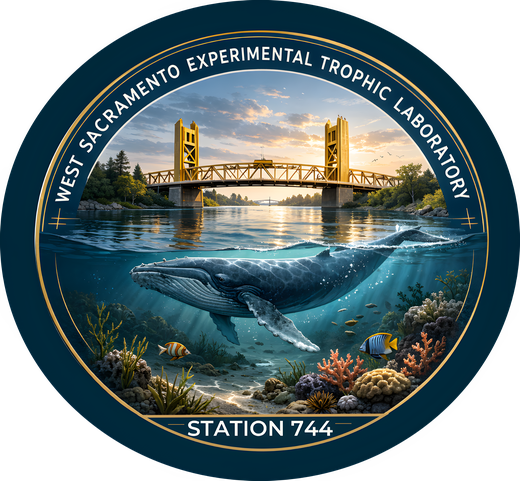
\includegraphics[width=1.00\linewidth]{../images/logo_small.png}
\end{minipage}\hfill
\begin{minipage}[c]{0.78\textwidth}
{\scriptsize\textbf{\color{agencyblue}W.E.T. LAB FIELD OPERATIONS UNIT}}\par
\vspace{2pt}
{\Large\bfseries\color{deepsea}Station 744 Plankton Survival Simulation}\par
\vspace{2pt}
{\small Water Column Buoyancy Trial | Photic Zone Residence Protocol}
\end{minipage}

\vspace{7pt}
{\footnotesize
\rowcolors{1}{titlebg}{white}
\begin{tabularx}{\textwidth}{@{}>{\bfseries\color{deepsea}}l Y >{\bfseries\color{deepsea}}l Y@{}}
Program & Plankton morphology and buoyancy testing & Status & Internal use only \\
Habitat target & Photic zone residence in the upper water column & Award & \$200 research funding \\
\end{tabularx}}
\end{tcolorbox}

\vspace{6pt}

\begin{minipage}[t]{0.485\textwidth}
\vspace{0pt}
\begin{labbox}{Study Objective}
Engineer a plankton body plan that remains suspended in the water column as long as possible without floating helplessly on the surface.
\end{labbox}

\begin{labbox}{Ecological Background}
\begin{itemize}
\item Plankton are drifting organisms too small to swim against current.
\item Phytoplankton photosynthesize and generate roughly 50\% of atmospheric oxygen.
\item Zooplankton graze on phytoplankton and support fish, crustaceans, mollusks, and baleen whales.
\item Both must remain in the sunlit photic zone, which extends to about 260 feet in the ocean.
\end{itemize}
\end{labbox}

\begin{labbox}{Experimental System}
\begin{itemize}
\item Research labs = teams
\item Clay core = plankton body
\item Craft add-ons = spikes, frills, and drag structures
\item Mason jar or bucket = water column
\item Sink time = survival score
\end{itemize}
\end{labbox}

\begin{labbox}{Protocol}
\begin{enumerate}
\item Build one plankton prototype using all clay provided.
\item Add approved craft materials to increase drag or trap air.
\item Release prototypes simultaneously into the water column and begin timing.
\item The winning design shows the slowest controlled descent to the bottom. Surface floaters are not successful plankton.
\end{enumerate}
\end{labbox}
\end{minipage}\hfill
\begin{minipage}[t]{0.485\textwidth}
\vspace{0pt}
\begin{labbox}{Survival Logic}
\begin{itemize}
\item Flat shapes and long spines increase surface area and slow sinking.
\item Trapped air and oil-like low-density pockets add buoyancy.
\item Stable, slow descent keeps plankton available for light, feeding, and survival in the food web.
\end{itemize}
\end{labbox}

\begin{labbox}{Design Inspirations}
Representative phytoplankton and zooplankton forms from the reference sink-off guide:

\vspace{4pt}
\begin{tabular}{@{}cc@{}}
\inspimg{../images/plankton_phyto_disc.jpg}{Disc phyto} & \inspimg{../images/plankton_phyto_spike.jpg}{Spined phyto} \\
[4pt]
\inspimg{../images/plankton_zoo_crustacean.jpg}{Crustacean zoo} & \inspimg{../images/plankton_zoo_daphnia.jpg}{Buoyant grazer} \\
\end{tabular}
\end{labbox}

\begin{labbox}{Observational Notes}
Record sink time, whether the design spins or tumbles, whether it traps bubbles, and which adaptations keep it suspended below the surface.
\end{labbox}

\begin{labbox}{Plankton Types}
\begin{tabularx}{\linewidth}{@{}>{\bfseries}l Y@{}}
Phytoplankton & Plant-like plankton that photosynthesize and produce food and oxygen. \\
Zooplankton & Animal plankton that feed on phyto and other tiny organisms in the water column. \\
\end{tabularx}
\end{labbox}
\end{minipage}

\vspace{6pt}

\begin{labbox}{Outcome}
Winning plankton demonstrates \textbf{maximum water-column residence time} through high drag, balanced buoyancy, and stable orientation. 
Award disbursement: \textbf{\$200 research funding}.
\end{labbox}

\vfill
\begin{center}
\footnotesize\color{agencyblue}\textbf{W.E.T. LAB | Station 744 | Internal Use Only}
\end{center}

\end{document}
